\documentclass[a0,portrait]{a0poster}

\usepackage[margin=3cm]{geometry}
\usepackage{multicol}
\columnsep=100pt
\columnseprule=1pt
\usepackage[svgnames]{xcolor}
\usepackage{palatino}
\usepackage{amsmath}
\usepackage{graphicx}
\usepackage{booktabs}
\usepackage[labelfont=bf]{caption}
\usepackage{amsfonts, amsmath, amsthm, amssymb}
\usepackage{wrapfig}
\usepackage{caption}
\usepackage[caption=false]{subfig}
\usepackage{textcomp}
\usepackage{bm}

\usepackage{pifont}
\usepackage{xcolor}
\definecolor{myblue}{RGB}{50,150,90}

\newcommand{\bi}{\item[\color{myblue}\ding{108}]} 

\begin{document}

\begin{minipage}[b]{0.3\linewidth}
\centering

\includegraphics[width=25cm]{../fig/umk.png}
\end{minipage}\hspace*{4cm}

\vspace{1cm}

\begin{minipage}[b]{\linewidth}
\veryHuge\centering\color{myblue} 
\begin{minipage}[b]{\linewidth}
\textbf{Ligand Dissociation Pathways in T4 Lysozyme L99A}
  \end{minipage}
\end{minipage}
\color{Black}\\[1cm]
\begin{minipage}[b]{\linewidth}
  \huge Sylwia Czach$^{1,2}$, Aleksander Oskroba$^{1}$, and Jakub Rydzewski$^1$ \\[1cm]
\large $^1$ Institute of Physics, Nicolaus Copernicus University, Grudziadzka 5, 87-100 Torun, Poland\\
\large $^2$ Department of Biochemistry, Nicolaus Copernicus University, Lwowska 1, 87-100 Torun, Poland\\
\end{minipage}

\vspace{1cm}

\begin{multicols}{2}
\large
  \section*{\huge\centering\color{myblue}How to Find an Exit Tunnel?}
\vspace*{1cm}
\begin{minipage}[b]{\linewidth}
  \centering
  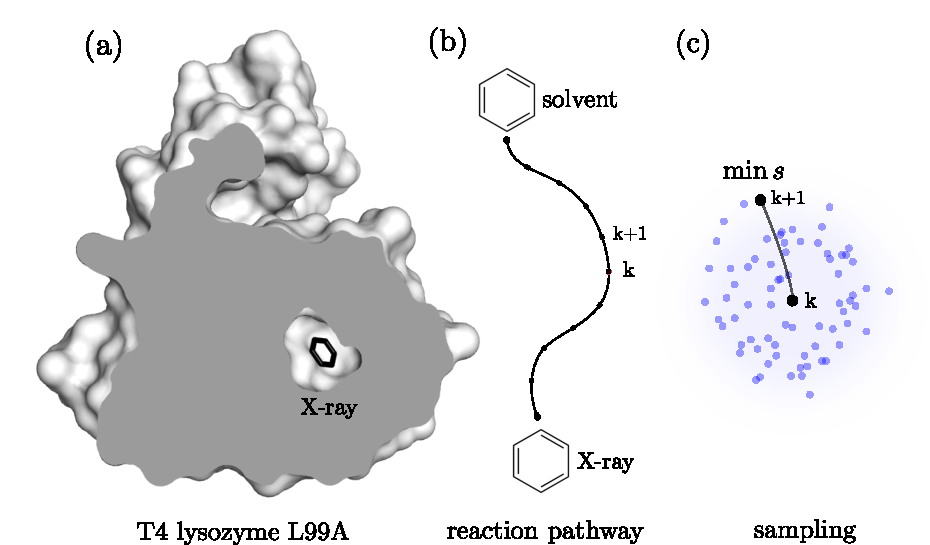
\includegraphics[width=32cm]{../fig/fig_1.pdf}
\end{minipage}

  \vspace{1cm}
\begin{minipage}[b]{\linewidth}
  
For each of $i$th pair of ligand-protein atoms the partial loss function is 
defined as $\exp(-r_i)/r_i$, where $r_i$ is the distance between the atoms 
and it is given by $r_i = \lambda \parallel x_k - y_l \parallel $

The loss function is the following:
\begin{equation}
    s = \sum^P_{i=1} \frac{\exp(-r_i)}{r_i},
\end{equation}
\vspace*{1cm}
where $P$ is the number of ligand-protein atom pairs.
    
\vspace*{1cm}
      
The loss function is optimized during MD simulations using the 
Metropolis–Hastings algorithm with the Boltzmann factors:
\begin{equation}
    p =  \left\{ \begin{array}{ll}
         \exp(-\beta (s(x')-s(x))) & \textnormal{ if } s(x') > s(x)\\
         1 & \textnormal{otherwise}
  \end{array} \right.
\end{equation}
where $x'$ is a randomly chosen neighboring position of the ligand 
and $\beta = 1/T(t)$ is a parameter introduced to decrease the 
probability of acceptance of a worse solution as the minimization 
procedure proceeds.
        
\end{minipage}

\begin{minipage}[b]{0.5\linewidth}
  \centering
  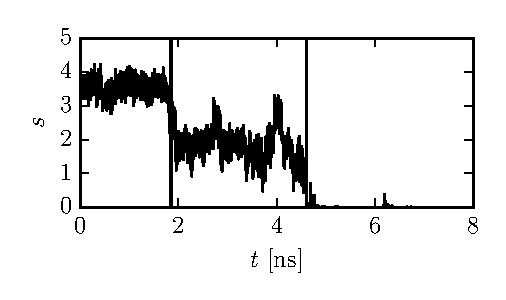
\includegraphics[width=20cm]{../fig/fig_2.pdf}
\end{minipage}
\hspace{1cm}
\begin{minipage}[b]{0.4\linewidth}
  \begin{itemize}
    \bi Enhanced sampling and non-convex optimization;
    \bi Biasing toward the minimum of the loss function;
    \bi Loss function describes interactions in a ligand-protein system;
  \end{itemize}
  \vspace*{1cm}
\end{minipage}

\section*{\huge\centering\color{myblue}Ligand Dissociation Pathways}
\vspace*{1cm}
\begin{minipage}[b]{\linewidth}
  \centering
  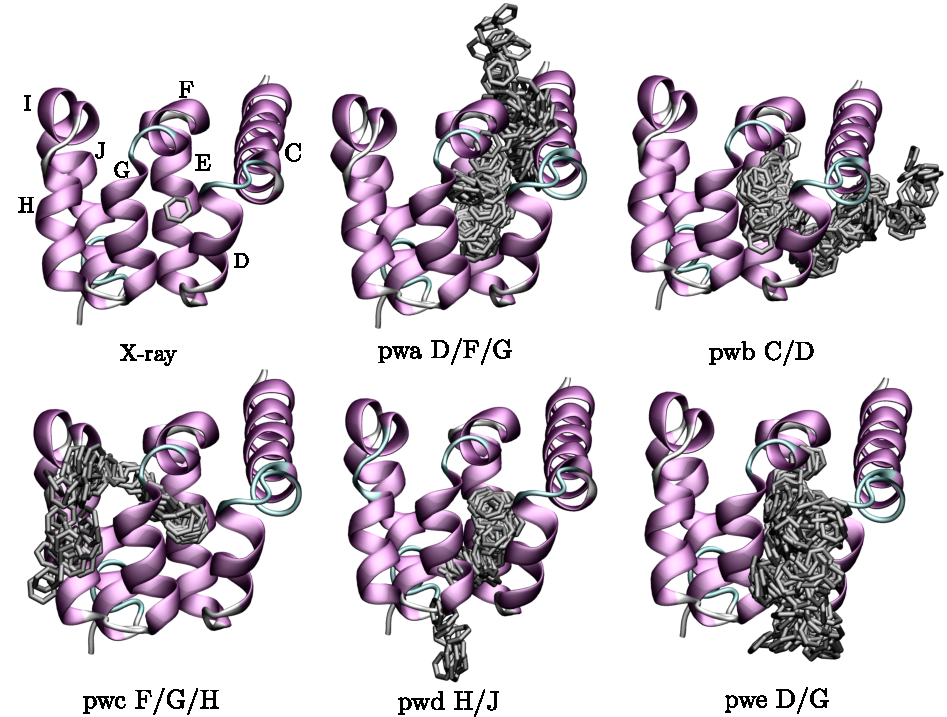
\includegraphics[width=38cm]{../fig/fig_3.pdf}
\end{minipage}

\section*{\huge\centering\color{myblue}Are Transient Pathways
  Heterogeneous?~\cite{3}}
\vspace*{1cm}
\begin{minipage}[b]{\linewidth}
  \centering
  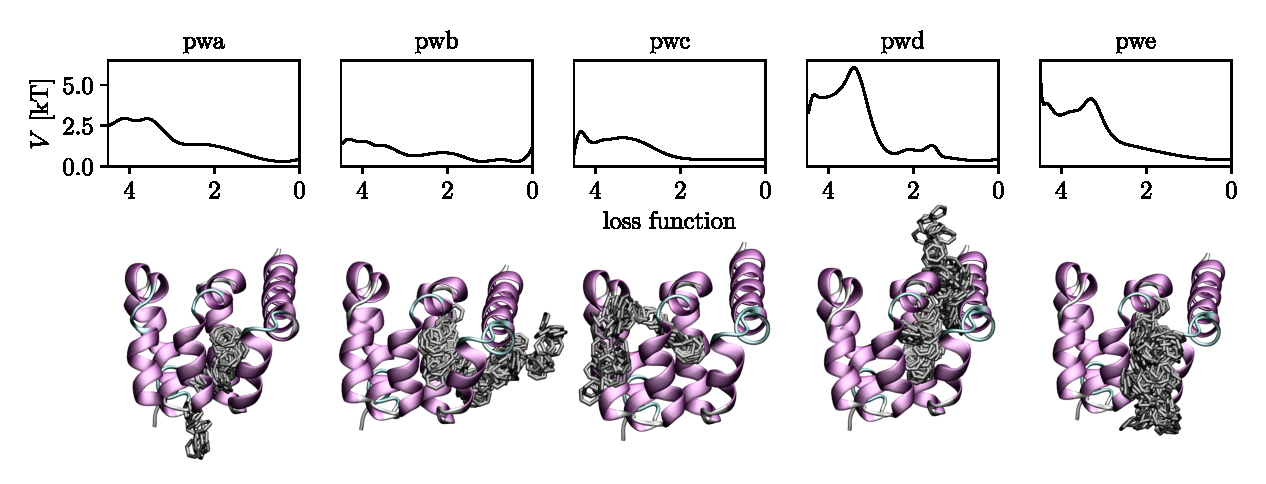
\includegraphics[width=36cm]{../fig/fig_4.pdf}
\end{minipage}

\noindent Reaction pathways of the benzene unbinding from the lysozyme L99A mutant
classified in five clusters.  In the upper panel the bias potential is shown as
a function of the minimized loss function. The bottom panel depicts
atomistically the reaction pathways.

\section*{\huge\centering\color{myblue}\texttt{maze}: A Module for Plumed
2~\cite{3}}
\vspace*{1cm}
\begin{minipage}[b]{\linewidth}
  \centering
  
\includegraphics[width=20cm]{../fig/maze-icon.png}
\end{minipage}
\vspace*{1cm}

\noindent\texttt{maze} is a code that implements enhanced sampling methods for simulating 
the reaction pathways of ligand unbinding. It is made as a module for Plumed 2, an
engine for free energy calculations of atomistic systems.
\vspace*{1cm}

\begin{minipage}[b]{0.5\linewidth}
  \centering
  
\includegraphics[width=12cm]{../fig/github.png}\\[1cm]
  \large Fork \texttt{maze} from Github.
\end{minipage}
\begin{minipage}[b]{0.5\linewidth}
  \centering
  
\includegraphics[width=12cm]{../fig/gitter.png}\\[1cm]
  \large Ask us on Gitter.
\end{minipage}

\color{myblue}
\begin{thebibliography}{6}%
\color{black}
\bibitem{1} J. Rydzewski, O. Valsson, \textit{J. Chem. Phys.} 150 (2019).
\bibitem{2} J. Rydzewski, \dots, H. Grubm\"{u}ller. \textit{J. Chem. Theory Comput.} 14, 2843 (2018).
\bibitem{3} J. Rydzewski, \textit{Submitted} (2019).
\end{thebibliography}
\color{black}

\section*{\color{myblue} Contact}
\begin{itemize}
    \bi Jakub Rydzewski \texttt{jr@fizyka.umk.pl}
\end{itemize}

\section*{\color{myblue} Acknowledgments}
This work is supported by the National Science Centre, Poland (grants
2016/20/T/ST3/00488 and 2016/23/B/ST4/01770). The MD simulations were computed
using facilities of Interdisciplinary Centre of Modern Technologies, Nicolaus
Copernicus University, Poland.
\\
\\
All the data and PLUMED input files required to reproduce the results reported in
this study will be available on PLUMED-NEST (\texttt{www.plumed-nest.org}), the public
repository of the PLUMED consortium. 

\end{multicols}
\end{document}
